% !TeX root = ../main.tex
% Add the above to each chapter to make compiling the PDF easier for some editors.

\chapter{Experiments}\label{chapter:experiments}

This thesis uses the BERTopic model to apply topic modeling on the \#Secim2023 dataset. 
Before diving into the results and discussion, this chapter explains the dataset, 
how the tweet hydration\footnote{The process of retrieving a tweet's complete information
with only tweet ID.} is performed on the tweets from the dataset, how BERTopic and 
neural topic modeling works generally.

\section{The Dataset}

The dataset published by \textcite{secim2023} consists of tweet IDs collected daily 
between July 2022 and June 2023, a total of around 250 million tweets. 
The frequency of the collected tweets is shown in \autoref{fig:collected_tweets}.

\begin{figure}[htb]
    \centering
    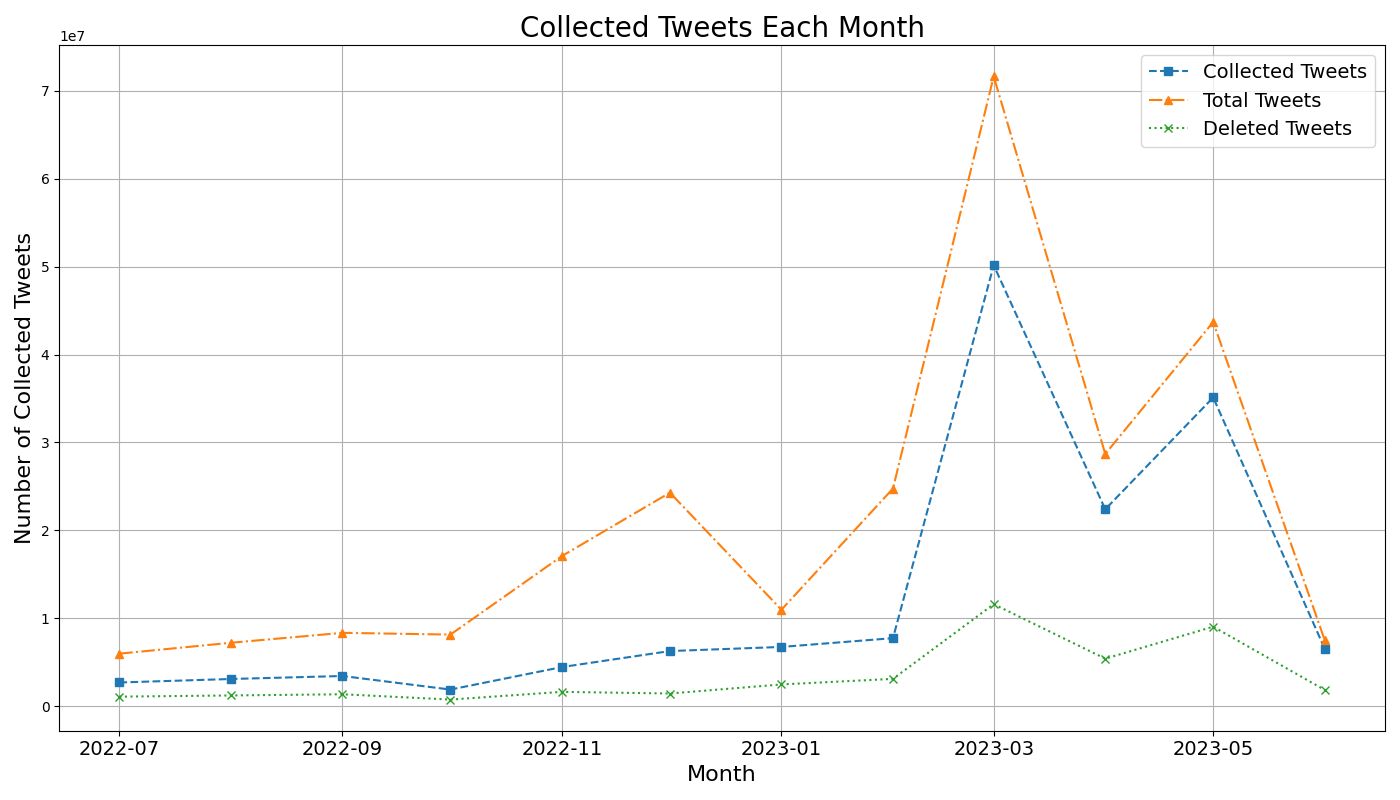
\includegraphics[width=\linewidth]{figures/collected_tweets_2.png}
    \caption[Collected Tweets each month]
    {Number of collected tweets from \#Secim2023 database monthly from July 2022 to June 2023.
    The orange line displays the total number of tweets in the database, 
    the blue line displays the total number of collected tweets from the database and 
    the green line displays the deleted tweets on the month of hydration, around
    December 2023.}\label{fig:collected_tweets}
\end{figure}

Due to Twitter's Developer Agreement and Policy\footnote{\url{https://developer.twitter.com/en/developer-terms/agreement-and-policy}}, 
a public dataset can only include (tweet) IDs. In order to access all tweet information,
they must be hydrated. Typically, a year before, a research group would have had access 
to Twitter Academic API\footnote{\url{https://developer.twitter.com/en/use-cases/do-research/academic-research}} 
and used packages like Hydrator\footnote{\url{https://github.com/DocNow/hydrator}} to gather 
tweet information quickly. Unfortunately, after Elon Musk bought Twitter, Academic API was 
restricted and then shut down at the end of May 2023 \parencite{calma_twitter_academicAPI_elon_2023},
before the start of this thesis. Today, there are only paid 
options starting from 100\$ for 10,000 tweets per month, 0.3\% of what was previously 
available for free access in a single day. 

If one has tweet IDs, other methods exist to hydrate the tweets nowadays. 
All of the following methods use some embedded retrieval mechanism to gather 
the tweet information. The first method uses Twitter's official page to 
retrieve embedded posts or videos given the tweet ID\@: \url{https://publish.twitter.com}. 
The second method, also used in this thesis, is implemented by React engineers in-house\@:
\url{https://github.com/vercel/react-tweet}. One can have a JSON output with sufficient 
information for analysis by sending HTTP requests and tweet ID as a parameter. 
As seen in \autoref{fig:collected_tweets}, the collected tweets (blue) are less than 
the total tweets in the dataset (orange). One of the main reasons for that is the deleted 
tweets. Since the hydration timeline for this thesis was between October 2023 and January 2024, 
and the tweets are between July 2022 and June 2023, there are approximately 50 million 
deleted tweets in the dataset (green). 

There are several reasons why there are lots of deleted tweets. The main reason for the 
vast number is the deletion of highly interacted original tweet posts. According to Twitter, 
if the original tweet is deleted, the reposts to that tweet are also not available 
anymore\footnote{\url{https://help.twitter.com/en/using-x/repost-faqs}}. 

Furthermore, the question of why people deleted their posts in the first place 
can be answered in two aspects. First, as mentioned in this New York Times article 
by \textcite{klosowski_delete_tweets_2022}, whether the person posting is a public figure 
or not is not essential\@: companies in the hiring process could run a social media 
background check, leading to rejection. Secondly and even worse, the government can pull 
an old tweet out of context and use it against the person, leading to an arrest. 
The Turkish government's control over social media is widely recognized. 
It has instituted nationwide bans before and has arrested people accused of 
``provocative posts'' continuously \parencite{scott_turkey_social_media_ban_2023}.
Freedom House's 2023 report states that Turkey's global and internet freedom scores are 
classified as ``not free'' \parencite{freedom-house_turkey_report}. 
These reasons could have eventually led to the deletion of many tweets 
after the election.

The gap between collected plus deleted tweets and total tweets lies under restricted 
rate limits\footnote{\url{https://business.twitter.com/en/blog/update-on-twitters-limited-usage.html}}. 
During hydration, every second or third response was empty, which led to second 
and third hydration batches of the missing tweets. Due to time limitations 
and the lengthy duration of big data analysis, the hydration process resulted in the 
maximum feasible collection of tweets within the constraints.

\section{The Methodology}

As mentioned in the previous chapter, topic modeling is an unsupervised tool that helps 
extract the underlying themes from the given text data. BERTopic is a neural topic model, 
one of many topic modeling approaches.
Due to time constraints and the time plan of this thesis, only the BERTopic model 
is used for topic modeling. Since several methods could be used, it is important 
to mention why BERTopic is used and why the others are not.
\textcite{topic_model_comparison_bertopic_2022} found out that for short and 
unstructured texts like Twitter data, BERTopic can extract contextual information, 
and it offers the most potential compared to different embedding-based topic models like Top2Vec.
According to their research, BERTopic has high versatility and stability across 
domains and supports different topic modeling variations. Like other embedding-based 
topic models, it allows multilingual analysis, and there is no need for 
preprocessing of the original data. However, the embedding approach might cause 
too many topics and outliers in some cases, which makes the results more 
challenging to interpret and should be examined in detail. 
Some long documents could occasionally involve multiple topics, but in this 
approach, every document is assigned to a single topic, which could be a 
disadvantage.

According to \textcite{bertopic}, BERTopic generates topic representations in six steps. 
First, without preprocessing, each document must be embedded using a pre-trained model. 
In this thesis, the SBERT model is used, introduced by \textcite{sentence-bert}. 
SBERT modifies the BERT model and derives semantically meaningful sentence embeddings, 
also from multilingual documents, allowing tasks like clustering or information retrieval 
via semantic search. SBERT also allows the selection of various pre-trained multilingual 
models supporting more than 50 languages\footnote{\url{https://www.sbert.net/docs/pretrained_models.html}}. 
This thesis uses the \textit{paraphrase-multilingual-MiniLM-L12-v2} model, which supports 
Turkish and is the fastest and one of the best performers among other multilingual models 
\parencite{reimers_sbert_multilingual_2020}. This part of the pipeline allows to do 
chunk embeddings, saving the results and using them later, making the big data analysis 
easier with restricted hardware availabilities.

Secondly, the dimensionality of these resulting embeddings is reduced to optimize the 
clustering process by the Uniform Manifold Approximation and Projection (UMAP) algorithm, 
which plays a massive role in big data analysis \parencite{mcinnes_umap_2020}. 
Afterward, these low-dimension embeddings are clustered using the Hierarchical Density-Based 
Spatial Clustering of Applications with Noise (HDBSCAN) technique, and the resulting 
clusters consist of semantically similar documents. This step allows unrelated documents 
to be assigned as noise or outliers, which improves the result, and both of these 
steps can be influenced very much by changing the parameters of the algorithms.

Fourthly, each cluster is tokenized using a Vectorizer like 
CountVectorizer\footnote{\url{https://maartengr.github.io/BERTopic/getting_started/vectorizers/vectorizers.html}}. 
Together with the weighting of these tokens, where a custom 
class-based variation of the Term Frequency -- Inverse Document Frequency (c-TF-IDF) algorithm 
is used, they are responsible for creating the topic representations. 
Like the previous step, this step also allows room to play with various parameters 
to tune the model, which affects the results considerably.

At last comes the topic representation, where the topics can be fine-tuned 
using various methods. This thesis uses KeyBERTInspired and Maximal Marginal Relevance (MMR) 
models\footnote{\url{https://maartengr.github.io/BERTopic/getting_started/representation/representation.html}}, 
which can be easily imported from the BERTopic library. They leverage the c-TF-IDF algorithm 
and weights keywords to represent the related topics. 
This thesis also leverages the power of LLMs by OpenAI, specifically GPT-4 Turbo, 
to better represent the resulting topics. One can also leverage other open-source LLMs, 
but most only support English or a few other languages.

% compare with Top2Vec
% advantages and disadvantages of BERTopic
% why aren't others used?
